\chapter{Sum Tree}\label{app:SumTree}

A sum tree is a binary search tree where each non-leaf node is the sum of it's
child nodes.
This was useful in the case of Prioritised Experience Replay as it reduces the
search time from order $O(n)$ to order $O(\log n)$.
Another useful property of the sum tree is that the root node is the sum of all
the leaf nodes, which is required to normalise the priority values into
probabilities.

Randomly sampling experiences with the correct distribution is achieved by first
sampling some value $r$ from uniform distribution, then navigating the tree
until a leaf node is reached, the index of the node corresponds to the index of
experience to be sampled.

Navigating the tree starts at the root node, the value $r$ is compared against
the left child node: if $r$ is less than the child node, then that node becomes
the current node; if not, the value of the child node is subtracted from $r$ and
the right child node becomes the current node.
If no left child node is present, the search is complete.

~\\
\underline{\textit{Example:}}

\noindent Consider the following tree:
\begin{center}
    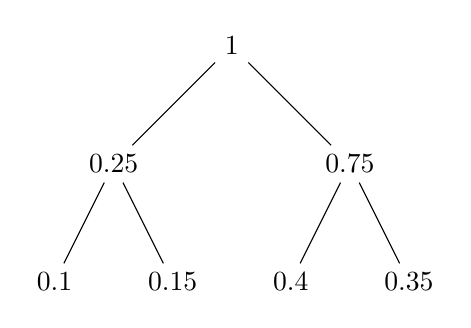
\begin{tikzpicture}
        [   grow = down
        ,   level/.style =
            {   sibling distance = 3cm/#1
            ,   level distance = 1.5cm
            }
        ]
        \node {1}
        child
        {   node {0.25}
            child
            {   node {0.1}
            }
            child
            {   node {0.15}
            }
        }
        child
        {   node {0.75}
            child
            {   node {0.4}
            }
            child
            {   node {0.35}
            }
        };
    \end{tikzpicture}
\end{center}
Suppose the value $r = 0.45$ is randomly generated from a uniform distribution:
$r$ is greater than the left child node, $0.25$, so subtract the left node value
and move to the right child node, $r \leftarrow r - 0.25 = 0.2$;
$r$ is less than the left child node, $0.4$, so move to the left child node;
no left child node is present, search complete;
search ended on the $3^\text{rd}$ leaf node, select the $3^\text{rd}$
experience from the replay memory.
